\documentclass[review]{elsarticle}

%New Ideas and Trends Paper
%https://www.journals.elsevier.com/journal-of-systems-and-software/news/jss-introduces-new-ideas-and-trends-papers
%Such a short paper is limited to 3000 words (approx. 5 pages, a figure counts as 200 words).

\usepackage{lineno,hyperref}

%%\usepackage{graphicx}
\usepackage[dvipdfmx]{graphicx}
%\usepackage{latexsym}
\usepackage{slashbox}
%\usepackage{multirow}
\usepackage{url}
\usepackage{color}
\usepackage{colortbl}
\usepackage{hhline}
\usepackage{flushend}
\usepackage{verbatim}
%\usepackage{hyperref}
\usepackage{enumerate}
\usepackage[sort&compress]{natbib}
\usepackage{subfigure}
\usepackage{framed}
%\usepackage{natbib}

\newcommand{\todo}[1]{{\color{green}{\textbf{TODO: [#1]}}}}
\newcommand{\yasu}[1]{{\color{red}{\textbf{Yasu says: [#1]}}}}
\newcommand{\emad}[1]{{\color{blue}{\textbf{[#1]}}}}
\newcommand{\Emad}[1]{{\color{blue}{\textbf{[#1]}}}}
\newcommand{\revised}[1]{{\color{red}{#1}}}
\newcommand{\para}[1]{{\color{magenta}{\textbf{This paragraph:}}} [#1]}

%\newcommand{\revised}[2]{\marginpar{\fbox{#2}}{\color{red}{#1}}}

\newcommand{\nbf}[1]{
%  \noindent{\textit{\textbf{#1}}}
  \noindent{\textbf{#1}}
}

\newcommand{\conclusionbox}[1]{%
	\vspace{2mm}
  \noindent
	\framebox[0.48\textwidth][c]{%
		\parbox[b]{0.45\textwidth}{%
			{\em #1}
		}
	}
}

% Set bibliography title
%\renewcommand\refname{REFERENCES}
%\renewcommand\bibsection{\section{\refname}}

\newcommand{\ea}{{\em et al.}}
\newcommand{\smallsection}[1]{\vspace{1mm}\noindent {\bf #1}.\hspace{2mm}}
\newcommand{\emphsection}[1]{\vspace{1mm}\noindent \underline{{\em #1}.}\hspace{2mm}}


% Reduce bibliography font size
%\def\bibfont{\normalsize} %normalsize should be default
% small or footnotesize

% Reduce space between references
%\setlength{\bibsep}{3.2pt} %3.5pt should be default

\usepackage{slashbox}
\usepackage{multirow}
\usepackage{color}

\newcommand{\todo}[1]{{\color{green}{\textbf{TODO: [#1]}}}}
\newcommand{\ea}{{\em et al.}}
\newcommand{\smallsection}[1]{\vspace{1mm}\noindent {\bf #1}.\hspace{2mm}}
\newcommand{\emphsection}[1]{\vspace{1mm}\noindent \underline{{\em #1}.}\hspace{2mm}}

\newcommand{\revised}[1]{{\color{red}{#1}}}
\newcommand{\conclusionbox}[1]{%
    \vspace{2mm}
  \noindent
    \framebox[0.96\textwidth][c]{%
        \parbox[b]{0.90\textwidth}{%
            {\em #1}
        }
    }
}


\modulolinenumbers[5]

\journal{Journal of Systems and Software: New Ideas and Trends Paper}

%%%%%%%%%%%%%%%%%%%%%%%
%% Elsevier bibliography styles
%%%%%%%%%%%%%%%%%%%%%%%
%% To change the style, put a % in front of the second line of the current style and
%% remove the % from the second line of the style you would like to use.
%%%%%%%%%%%%%%%%%%%%%%%

%% Numbered
%\bibliographystyle{model1-num-names}

%% Numbered without titles
%\bibliographystyle{model1a-num-names}

%% Harvard
%\bibliographystyle{model2-names.bst}\biboptions{authoryear}

%% Vancouver numbered
%\usepackage{numcompress}\bibliographystyle{model3-num-names}

%% Vancouver name/year
%\usepackage{numcompress}\bibliographystyle{model4-names}\biboptions{authoryear}

%% APA style
%\bibliographystyle{model5-names}\biboptions{authoryear}

%% AMA style
%\usepackage{numcompress}\bibliographystyle{model6-num-names}

%% `Elsevier LaTeX' style
\bibliographystyle{elsarticle-num}
%%%%%%%%%%%%%%%%%%%%%%%

\begin{document}

\begin{frontmatter}

\title{Using Analytics to Quantify the Interest of Self-Admitted Technical Debt}
%\tnotetext[mytitlenote]{Fully documented templates are available in the elsarticle package on \href{http://www.ctan.org/tex-archive/macros/latex/contrib/elsarticle}{CTAN}.}

%% Group authors per affiliation:
\author[kyushu]{Yasutaka Kamei\corref{mycorrespondingauthor}}
\cortext[mycorrespondingauthor]{Corresponding author}
\ead{kamei@ait.kyushu-u.ac.jp}
%\fntext[myfootnote]{Since 1880.}

\author[concordia]{Everton Maldonado}

%% or include affiliations in footnotes:
\author[concordia]{Emad Shihab}

\author[kyushu]{Naoyasu Ubayashi}

\address[kyushu]{Principles of Software Languages Group (POSL), Kyushu University, Fukuoka, Japan}
\address[concordia]{Data-driven Analysis of Software (DAS) Lab , Concordia University, Montre\'al, Canada}

\begin{abstract}
This template helps you to create a properly formatted \LaTeX\ manuscript.
\end{abstract}

\begin{keyword}
\texttt{elsarticle.cls}\sep \LaTeX\sep Elsevier \sep template
\MSC[2010] 00-01\sep  99-00
\end{keyword}

\end{frontmatter}

\linenumbers

%What is technical debt and self-admitted technical debt
\section{Introduction}
Technical debt was first coined by Cunningham in 1992 to refer to the phenomena of taking a shortcut to achieve short term development gain at the cost of increased maintenance effort in the future \cite{Cunningham1992WPM}. The technical debt community, organized through the managing technical debt workshop \cite{MTD2016}, has studied many aspects of technical debt, including its detection \cite{Zazworka2013EASE}, impact \cite{Zazworka2011MTD} and the appearance of technical debt in the form of code smells \cite{Fontana2012MTD}. Most recently, we developed an approach to identify technical debt from code comments, referred to as self-admitted technical debt (SATD). SATD refers to the situation where developers know that the current implementation is not optimal and write comments alerting the inadequacy of the solution. 

% What people did and what is the impact of TD. What they found.
In the last few years, an increasing amount of work has focused on SATD. In particular, our prior work focused on the detection of SATD~\cite{Potdar2014ICSME,Maldonado_TSE2017} and the classification of different types of SATD and the development of datasets to enable future studies on SATD~\cite{Maldonado2015MTD}. Other work by Bavota and Russo~\cite{Bavota2016MSR} performed an empirical study of SATD on a large number of Apache projects showed that SATD is prevalent in open source projects, is long lived and is increasing over time. A study by Wehaibi et al.~\cite{Wehaibi2016SANER} examined the impact of SATD on quality and found that SATD does not necessarily relate to more defects, however, it does make the software system more complex. 

%However, very little work focused on interest. Also, why is calculating interest difficult
Although the metaphor of technical debt has been well studied, to the best of our knowledge, the cost of debt/interest has not been extensively studied. Measuring the interest of the technical debt is one of the challenges in the field, since it requires for the detection of the technical debt, the tracking of the debt over time and the development of measures to accurately quantify this debt. Given that SATD allows us to know the exact method the technical debt exists in, we are able to perform fine-grained analysis of the code, which enables us to quantify interest of the debt. In this paper, the interest refers to the additional difficulty in repaying the debt.

We investigate the use of code metrics, in particular the well-known Lines of Code (LOC) and Fan-In, to measure interest. We use LOC since it highly correlates with most code complexity metrics and Fan-In\footnote{{\sc Understand} calculates Fan-In as the number of inputs a function uses plus the number of unique subprograms calling the function~\cite{FANIN}.} since it allows us to measure how much a piece of code is depended on by other code. Then, we use the developed measure to determine how much of the SATD incurs positive interest. 
%In a case study on the Apache JMeter project, we find that using LOC, 44.2\% and using Fan-In 42.2\% of the SATD in JMeter incurs positive interest.

\revised{This paper is an extended version of our earlier workshop paper~\cite{Kamei2016TDA}. We extend our previous work by:}

\revised{
\begin{itemize}
\item We use the state-of-art approach~\cite{Maldonado_TSE2017}, which has been recently published, based on natural language processing to detect SATD.
\item We conduct our case study using the data sets that are collected from five open source software projects.
\item We perform deeper analysis to discuss (1) what is the difference  between the interest of SATD and non-SATD (2) how the SATD that incurs large positive interest is introduced in development process.  
\end{itemize}
}

% Organization of the paper
The rest of the paper is organized as follows; Section \ref{sec:approach} introduces our approach to quantify interest of SATD. Section \ref{sec:results} describes a study using the developed measure and Section \ref{sec:discussion} presents our discussion. Finally, Section \ref{sec:conclusion} draws conclusions and our future work.

%-----------------------------------------------------------------------
\begin{figure*}[!t]
  \begin{center}
  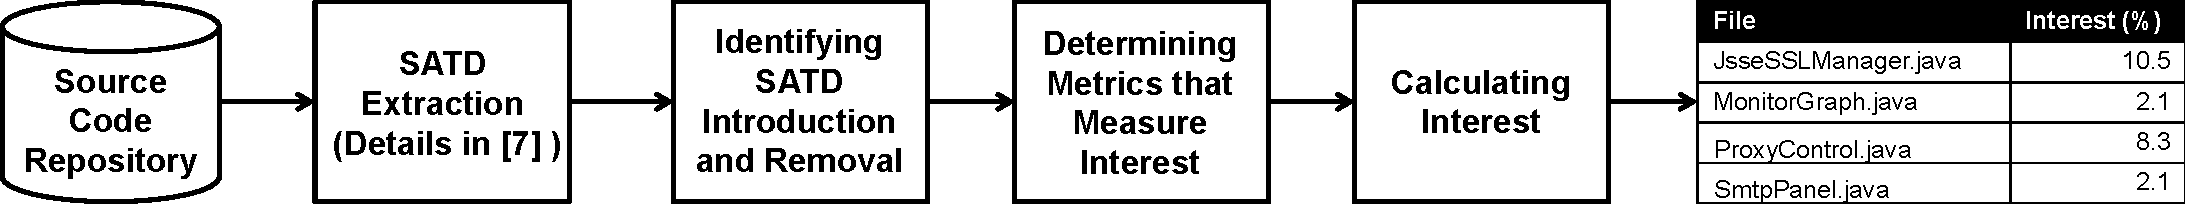
\includegraphics[width=.95\textwidth]{figures/overview}
  \caption{The overview of our approach.}
  \label{fig:overview}
  \end{center}
\end{figure*}
%-----------------------------------------------------------------------

\section{Approach} \label{sec:approach}

\smallsection{1. SATD Extraction}
In order to measure interest of the TD, our first step is to identify where it exists. Since we focus particularly on SATD, we use code comments found in the source code. 

\todo{We explain the TSE approach here}.~\cite{Maldonado_TSE2017}

% \todo{We need to ask Everton about git commonds to find where it was introduced and removed.
\smallsection{2. Identifying SATD Introduction and Removal}
Since we are interested in measuring the interest, we need to determine the `change' over time in these SATD methods. For each of the SATD comments identified by us, we use several git commands (e.g., {\tt git log -- <PATH\_TO\_FILE>} and {\tt git cat-file <SHA1>:<PATH\_TO\_FILE>}), to trace a comment back to the commit where it was introduced. We perform this task by replaying the history commit-by-commit. Using the same technique, we are also able to detect the removal of SATD. We detect the removal of SATD when we find that the commit is removed or changed. 

\smallsection{3. Determining Metrics that Measure Interest}
Once we are able to determine the SATD comments and their associated methods, we would like to calculate the interest that is incurred over time (i.e., from the introduction of the technical debt to its removal). To do so, we extracted 16 code metrics using the {\sc Understand Tool}~\cite{Understand}. In particular, we selected all method-level complexity and size metrics that Understand is able to provide.

The reasons that we focused on complexity and size metrics are: 1) our intuition tells us that if a piece of code is introduced and then becomes more complex, then that is a good proxy for it being more difficult to deal with in the future, i.e., it incurred interest; and 2) prior work has shown that size metrics are typically highly correlated with complexity metrics, hence, we figured using size metrics (if they are highly correlated with complexity metrics in our case) would be an easier alternative to using complexity metrics.

We measured the Spearman correlation between the complexity and size metrics and found that indeed all metrics except Fan-In are highly correlated with LOC. Therefore, we decided to use the LOC metric as a measure of interest. In addition, since Fan-In is an indicator of how much a method is depended on, we decided to also include the Fan-In metric when calculating interest. The intuition being that if a method is depended on lightly when the SATD is introduced and then has many more dependencies in the future, then dealing with this SATD is much more difficult (since many dependencies may be affected). In the end, we settled on using the two metrics, LOC and Fan-In, as measures of interest.

%To calculate interest, we measure product metrics from two versions detected in Step 2 using {\sc Understand}~\cite{Understand}. We choose all metrics (e.g., LOC and Cyclymatic Complexity) that are available at the method-level in {\sc Understand}.

\begin{table}[tb]
  \caption{The Percentage of SATD that has Positive, Negative and No Change in Interest}
  \label{tab:percentage}
  \centering

  \begin{tabular}{cc|p{0.65in}|rrr}
  \hline
        & & \textbf{\# SATD instances} & \textbf{Positive} & \textbf{Negative} & \textbf{No Change} \\
  \hline
\multirow{2}{*}{Ant} &  LOC  & \multicolumn{1}{r|}{354} &  31.1\%  &  12.7\% & 56.2\%\\
                   & Fan-In  & \multicolumn{1}{r|}{332} &  23.5\%  &  10.8\% & 65.7\%\\
  \hline
\multirow{2}{*}{Hadoop} &  LOC  & \multicolumn{1}{r|}{370} &  28.4\%  &  11.1\% & 60.5\%\\
                      & Fan-In  & \multicolumn{1}{r|}{360} &  28.1\%  &  12.5\% & 59.4\%\\
  \hline
\multirow{2}{*}{JMeter} &  LOC  & \multicolumn{1}{r|}{460} &  25.9\%  &  19.8\% & 54.3\%\\
                      & Fan-In  & \multicolumn{1}{r|}{425} &  29.2\%  &  9.6\% & 61.2\%\\
  \hline
\multirow{2}{*}{Log4j} &  LOC  & \multicolumn{1}{r|}{65} &  10.8\%  &  9.2\% & 80.0\%\\
                     & Fan-In  & \multicolumn{1}{r|}{57} &  19.3\%  &  8.8\% & 71.9\%\\
  \hline
\multirow{2}{*}{Tomcat} &  LOC  & \multicolumn{1}{r|}{655} &  20.6\%  &  12.1\% & 67.3\%\\
                      & Fan-In  & \multicolumn{1}{r|}{623} &  21.5\%  &  9.8\% & 68.7\%\\
  \hline
  \end{tabular}
\end{table}

\smallsection{4. Calculating Interest}
Using our metrics, we consider the relative LOC and Fan-In values between the introduced and removed versions as interest. We calculate the interest per SATD instance. For example, if arbitrary metric values in the introduced and removed versions are 10 and 20 in the method where the SATD exists, the relative size is 100 (i.e, $100* \frac{(20-10)}{10}$). In cases where the SATD is not yet removed, we use the numbers from the latest version of JMeter. Our assumption here is that if the SATD incurs positive interest, then it will be more difficult to remove in the future, e.g., if the code becomes more complex compared to when the debt was taken, then it will be more difficult to deal with.

While the paper tackles the research topic that accelerates a new research direction (i.e., quantifying interest of SATD), it also has the weakness of our current approach. We elaborate on the weakness of our current approach in Section \ref{conclusion}.


\section{Case Study} \label{sec:results}
\smallsection{Motivation}
There exist several previous studies that focused on understanding SATD (e.g., the detection of technical debt~\cite{Potdar2014ICSME,Zazworka2013EASE} and the impact of SATD on software quality~\cite{Wehaibi2016SANER}). However, there are no studies that help in the quantification of SATD interest. Therefore, we would like to know how we can measure interest and if SATD actually incurs positive interest.

\smallsection{Approach}
To calculate interest of SATD, we follow the approach we explained in Section \ref{sec:approach}.
We show the number of SATD, the percentage of the technical debt that has positive interest, and the distribution of interest for technical debt that incurs an positive interest rate.

\smallsection{Datasets}
To conduct our case study, we collect data from six open source software projects (Apache Ant, Hadoop, JMeter, Log4j, Tomcat). All of them use Git as the version control system, which many of our tools are designed to work on. 
\todo{We need to know the updated information: In particular, we use release v2.10 of JMeter, which contains 81,307 SLOC in 1,181 classes, contains 20,084 comments, and has 33 unique contributors.}

\smallsection{Results}

\begin{table}[tb]
  \caption{Statistics of the SATD that incurs a positive rate}
  \label{tab:statistic}
  \centering

  \begin{tabular}{cc|rrrrr}
  \hline
        & \textbf{Min.} & \textbf{1st Qu.} & \textbf{Median} & \textbf{3rd Qu.} & \textbf{Max.} \\
  \hline
\multirow{2}{*}{Ant} &    LOC  & 0.6 &  5.9  &  16.5  &  35.8  &  157.4 \\
                     & Fan-In  & 4.0 & 20.3  &  33.3  &  78.8  &  600.0 \\
  \hline
\multirow{2}{*}{Hadoop} & LOC  & 0.3 &  8.7  &  25.0  &   57.1 &  283.3 \\
                     & Fan-In  & 2.9 & 20.0  &  40.0  &  100.0 &  666.7 \\
  \hline
\multirow{2}{*}{JMeter} & LOC  & 0.5 &  6.7  &  18.2  &   49.5 &  200.0 \\
                     & Fan-In  & 5.9 & 16.7  &  29.7  &   63.5 &  500.0 \\
  \hline
\multirow{2}{*}{Log4j} &  LOC  &  4.7 &  29.5 &  40.7  &   52.7 &   63.4 \\
                     & Fan-In  & 11.1 &  27.6 &  50.0  &  100.0 &  200.0 \\
  \hline
\multirow{2}{*}{Tomcat} & LOC  & 0.4 &  5.3  &  13.6  &   38.7 &  433.3 \\
                     & Fan-In  & 2.0 & 16.7  &  28.6  &   66.7 &  469.2 \\
  \hline
  \end{tabular}
\end{table}

\conclusionbox{
10.8\%--31.1\% of technical debt incurs a positive rate in terms of LOC and 19.3\%--28.1\% of technical debt incurs it in terms of Fan-In.}

\section{Discussion} \label{sec:discussion}
\subsection{SATD vs. Non-SATD}
Generally speaking, software systems are always evolving over time for implementing new functionality and fixing defects~\cite{Robles_IWPSE2005}.
Therefore, even if the size of technical debt increases, it is not clear about how the nature of software evaluation affects the interest of technical debt.
We would like to compare the impact of software evolution on methods in two groups of SATD v.s. non-SATD.


\begin{table}[tb]
  \caption{The Percentage of Non-SATD that has Positive, Negative and No Change in Interest}
  \label{tab:percentage_non-SATD} 
  \centering

  \begin{tabular}{cc|p{0.65in}|rrr}
  \hline
        & & \textbf{\# non-SATD instances} & \textbf{Positive} & \textbf{Negative} & \textbf{No Change} \\
  \hline
\multirow{2}{*}{Ant} &  LOC  & \multicolumn{1}{r|}{5,273} &  14.8\%  &  6.8\% & 78.4\%\\
                   & Fan-In  & \multicolumn{1}{r|}{4,924} &  8.6\%  &  5.1\% & 86.3\%\\
  \hline
\multirow{2}{*}{Hadoop} &  LOC  & \multicolumn{1}{r|}{11,247} &  11.0\%  &  4.8\% & 84.2\%\\
                      & Fan-In  & \multicolumn{1}{r|}{10,712} &  17.6\%  &  6.9\% & 75.5\%\\
  \hline
\multirow{2}{*}{JMeter} &  LOC  & \multicolumn{1}{r|}{8,116} &  12.9\%  &  13.1\% & 74.0\%\\
                      & Fan-In  & \multicolumn{1}{r|}{7,566} &  16.4\%  &  6.6\% & 77.0\%\\
  \hline
\multirow{2}{*}{Log4j} &  LOC  & \multicolumn{1}{r|}{1,387} &  11.5\%  &  5.9\% & 82.6\%\\
                     & Fan-In  & \multicolumn{1}{r|}{1,225} &  14.0\%  &  7.3\% & 78.7\%\\
  \hline
\multirow{2}{*}{Tomcat} &  LOC  & \multicolumn{1}{r|}{17,769} &  6.7\%  &  4.6\% & 88.7\%\\
                      & Fan-In  & \multicolumn{1}{r|}{16,487} &  11.0\%  &  5.0\% & 84.0\%\\
  \hline
  \end{tabular}
\end{table}


\smallsection{Approach}
We compare the interest of methods between SATD and non-SATD.
We conduct the following steps:
\begin{itemize}
\item [Step 1] We obtain the list of files that include SATD. % from technical_debt_summary.csv
\item [Step 2] We extract methods that do not include SATD in the files that we obtained in Step 1. % see .method-level.product.csv
\item [Step 3] We measure metrics for the methods that we extracted in Step 2 at two versions that technical debt is introduced and removed. We only use the methods that can be found at the two versions.
\item [Step 4] We calculate interest using metrics measured in Step 3.
\end{itemize}
% What do we need to do some pre-condition for this analysis?

\smallsection{Result}
Comparing the results of SATD (Table \ref{tab:percentage}) with non-SATD (Table \ref{tab:percentage_non-SATD}), we find that the positive rate of interest for SATD is larger than non-SATD in all cases except Log4j in according to LOC. We believe that this is one of evidense that SATD is likely to incur positive interest than non-SATD.

\begin{table}[t]
  \caption{The Percentage of Software Development Activities when SATD is Introduced/Removed}
  \label{tab:percentage_activities} 
  \centering

  \begin{tabular}{l|r|r|p{2.80in}}
  \hline
       \textbf{Reason} & \textbf{Intro} & \textbf{Removal} & \textbf{Examples} \\
  \hline
  Documentation & 2\%  &   4\% &  \textit{Starting the long road of javadoc updates} (jmeter -- 71f6e34), \textit{Better documentation.} (tomcat -- b51444a) \\
  Fix issues  &  18\%  &  23\% &  \textit{fix sizing issue when db is restarted fix JMX domain name fix exception handling} (tomcat -- 525865e). \\
  New Feature &  36\%  &   8\% &  \textit{HADOOP-9035. Generalize setup of LoginContext (daryn via bobby)} (hadoop -- 86ce5f6) \\
  Performance &   4\%  &   4\% &  \textit{Do not use Reader and Writer classes for writing response, because [...]} (jmeter -- f88f44b) \textit{HDFS-3726. [...] This isn't critical for correctness but will help reduce log spew on both sides.} (hadoop -- cae8116) \\ 
  Refactoring &  30\%  &  54\% &  \textit{moved some code within the acivation area into new methods.} (log4j -- 765875d) \\
  Testing     &   6\%  &   8\% &  \textit{Correctly define the ROOT context in unit tests} (tomcat -- a2153a3) \\
  Others      &   4\%  &   0\% &  \textit{Sometimes my brain just breaks...} (jmeter -- 5c21be0) \\
  \hline
  \end{tabular}
\end{table}

\subsection{Manual Analysis}
\smallsection{Motivation}
The interest varies among technical debt. If we can understand the reason why some of technical debt has large interest, we can make use of such insights for future development. Therefore, in this RQ, we would like to manually investigate why some of technical debt has large interest.

\smallsection{Approach}
To understand why technical debt is removed, we manually inspect commit messages that introduce and remove technical debt. We choose the top 50 SATD by sorting SATD by interest in decreasing order.

%To highlight the characteristics of technical debt that has large interest, we compare low interest technical debt with high interest technical debt.

\smallsection{Results}
Table \ref{tab:percentage_activities} shows the classification we conducted for top 50 SATD.
New feature is top development activities in according to SATD introduction. When developers implement new feature, they are not likely to finish implementing the new feature by one commit because of time pressure. The developers often mention "TODO" or other words for the part where they will work later. For example, the commit dbecbe5 in the Hadoop project, which implements MapReduce 2.0, adds SATD "// TODO gross hack". The developer notices that the implementation is not perfect, but conducts such workaround to save his/her development time.

Interestingly, refactoring is the top development activities when SATD is removed. When developers actually work on refactoring, they also fix SATD. For example, the commit c77f96a, which is categorized as refactoring, in the Tomcat project mentions "Drop tomcat-lite module. It never saw a release and has not seen meaningful development for over 4 years. "

\subsection{Threats to Validity} 
\todo{discuss threats to validity}

\section{Conclusion} \label{sec:conclusion}

\section*{References}

\bibliography{reference}

\end{document}